\chapter{Analysis}\label{chap:analysis}

This chapter describes the problem that this thesis addresses, as well as some existing solutions. It also specifies the functional and non-functional requirements of the system to be implemented to address the problem and some of the platforms it will be implemented on.

\section{Problem Analysis}
The problem of real-time communication is increasingly important as bandwidth and connections speeds increase, allowing for more interactivity between users and computer systems. More and more systems require increasing amounts of communication in this age of and ever increasing number of web-based applications taking the place of traditional desktop ones. With services feeding customized content to a large number of different users in a more interactive and immediate manner, traditional methods prove too slow and cumbersome.

However, not only user-to-user and user-to-machine interactions are increasing greatly, a massive growth has occurred in machine-to-machine communication due to more automation, usage of microservices, system distribution and software and platform provided as a service (SaaS and PaaS respectively).

These developments have led to changing requirements in the speed, volume and reliability in data delivery. The need has risen for fast and lightweight and secure real-time communication solutions.

The main difference between a traditional and realtime client-server\footnote{Please note that client-server terminology is meant as someone who connects (client) to someone who provides data (server). The client can be another server-side application.} communication is that traditionally, the server would respond to a request from the client, be it synchronously or asynchronously. This communication happens over what is basically a one way channel. When the client would expect new data from the server, it would poll at intervals for new data. 

During realtime communication on the other hand, a two way channel is kept open between the client and server and data is send and received both ways when needed, usually in an asynchronous fashion. See Figures ~\ref{fig:traditional-communication} and ~\ref{fig:realtime-communication-pattern}.

\begin{figure}[H]
	\centering
	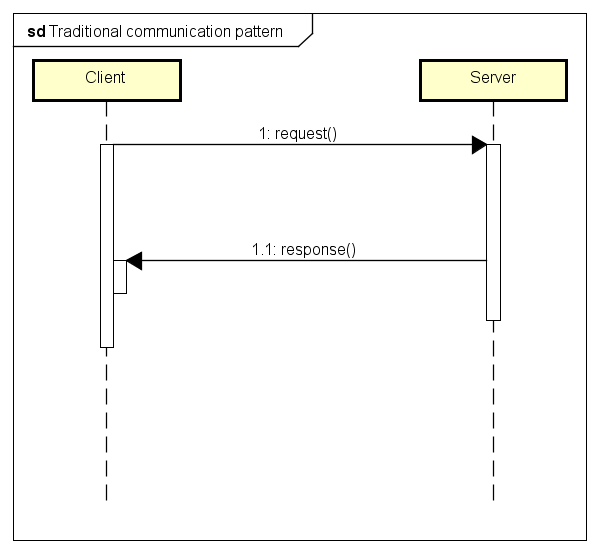
\includegraphics[width=0.65\textwidth]{figures/02_analysis/Traditional-communication-pattern}
    \caption{Traditional client-server communication pattern}
    \label{fig:traditional-communication}
\end{figure}

\begin{figure}[H]
	\centering
	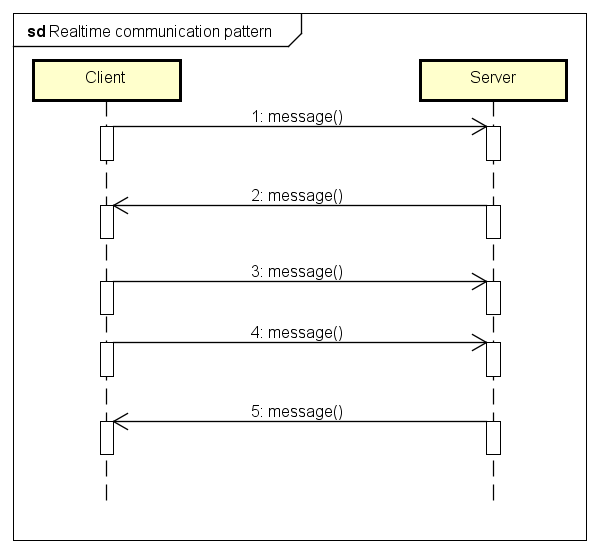
\includegraphics[width=0.65\textwidth]{figures/02_analysis/Realtime-communication-pattern}
    \caption{Realtime client-server communication pattern}
    \label{fig:realtime-communication-pattern}
\end{figure}

While the basic pattern appears simple, the situation complicates quickly once taken into account, that systems need to deliver realtime data to a large number of devices, often running on different platforms (eg. iOS and Android apps) and during periods of non-connectivity, such as a mobile device losing reception. 

A very simple example of such a situation can be seen in Figure ~\ref{fig:example-situation}. A service needs to send two different messages to two groups of users, that are using different platforms and some of them even have multiple devices at once (eg. an iPad and Android phone) and the message needs to be delivered to all of these. For simplicity, Figure ~\ref{fig:example-situation} only illustrates a one way message delivery, but for true interactivity such a system must be able to also receive data, not just send it.

\begin{figure}[H]
	\centering
	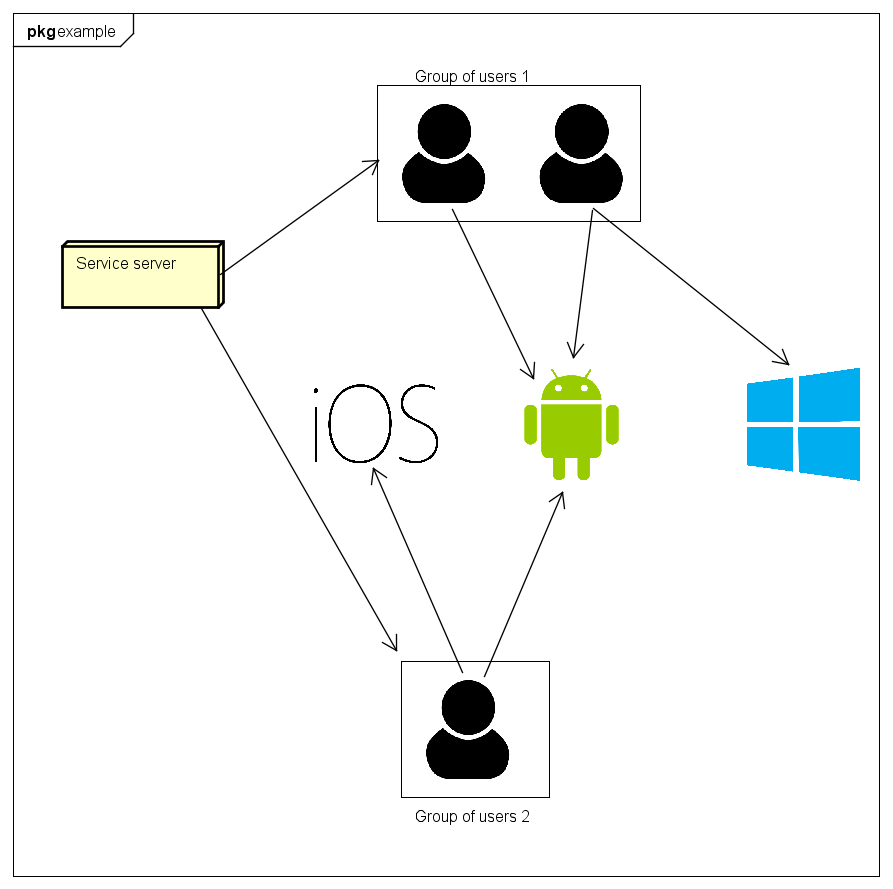
\includegraphics[width=0.8\textwidth]{figures/02_analysis/example-situation}
    \caption{Example situation of message delivery}
    \label{fig:example-situation}
\end{figure}

\section{Existing Similar Solutions} \label{sec:similar-solutions}
At the moment there are several products on the market that provide messaging with differing capabilities and pricing strategies.

Henceforth will be described an overview of some of the most popular ones at the time of writing, based on information provided in marketing materials, documentations and FAQs\footnote{Frequently Asked Questions}. An in-depth comparison of the inner workings of these is very hard, since they all operate on a closed-source basis and do not disclose much information regarding the inner workings of their algorithms and data structures. Furthermore, they are all provided as a service, without a possibility of self-deployment.

\subsection{PubNub}
PubNub\footnote{PubNub <\url{https://www.pubnub.com/}>} is a commercial realtime messaging service based on a Publish-Subscribe pattern. One of the largest messaging service providers in the world, PubNub boasts, among others, secure end-to-end encryption, unlimited number of channels and 250ms latencies worldwide~\protect\cite{pubnub-messaging} and with over 70+ SDKs\footnote{PubNub SDK full list <\url{https://www.pubnub.com/docs}>} can be used on virtually any platform.

Key features:
\begin{itemize}
\item Unlimited Publish/Subscribe channels~\protect\cite{pubnub-messaging} (technically, though device and message amounts are limited with tier-based pricing)
\item 250ms latency worldwide~\protect\cite{pubnub-messaging}
\item Push notification support for Android, iOS and Windows
\item Message delivery once target device comes online (catch-up) as long as message is still in queue. Messages are held in the queue by default for approximately 5 minutes or 100 messages, but can be extended using Storage add-on.~\protect\cite{pubnub-catchup}
\end{itemize}

Pricing\footnote{As of January 3 2018} (monthly):
\begin{itemize}
\item Free: allows 100 daily active devices and 1 million total messages
\item \$49: 500 devices
\item \$149: 1 500 devices
\item \$399: 5 000 devices
\item \$799: 20 000 devices
\end{itemize}

\subsection{Ably}
Ably\footnote{Ably <\url{https://www.ably.io/}>} is a commercial realtime data delivery platform based on a Publish-Subscribe pattern. Apart from several client libraries including ones for Javascript, Java, Python, PHP and others\footnote{Ably Download<\url{https://www.ably.io/download}>}. Ably provides WebSocket and REST based APIs.~\protect\cite{ably-docs} Like PubNub, Ably also provides secure end-to-end encryption.

Key features:
\begin{itemize}
\item Presence awareness, ie. notification when a device becomes online or offline
\item Access to channel message history where messages are stored for 24-72 hours~\protect\cite{ably-history} with persisted history enabled, or 2 minutes otherwise
\item Binary encoded messages help reduce bandwidth and streamlines processing time for encoding and decoding messages~\protect\cite{ably-bin-enc}
\item Message and worker queues
\item Reliable message ordering~\protect\cite{ably-order} - devices are guaranteed to receive messages in the order they were sent
\item WebHooks
\item Simple WebSocket and REST APIs allow for easy client implementation for platforms other than officially supported
\item Protocol adapters providing interoperability between other realtime and queuing protocols~\protect\cite{ably-adapters}
\end{itemize}

Pricing\footnote{As of January 3 2018}:

Unlike PubNub's tier-based monthly pricing system, Ably provides a more flexible monetization model:
\begin{itemize}
\item Free: 100 peak connections and channels, 3 million monthly messages
\item Self-service: \$12.50 per thousand peak connections or channels, \$1.25 per million messages, volume discounts
\item Enterprise: tailored package with premium support and no hard limits
\end{itemize}

\subsection{Pusher}
Pusher\footnote{Pusher <\url{https://pusher.com/}>} is a commercial realtime messaging service based on a Publish-Subscribe pattern. Pusher provides WebSocket and HTTP APIs for message publishing. Like all previously mentioned services, Pusher also supports end-to-end encryption.

Pusher also provides SDKs for both sending and receiving messages for several languages and frameworks including Go, Java, Node.js, Javascript, Swift, PHP, Python and others\cite{pusher-libs}. 

There is also a range of community developed and maintained libraries including languages and frameworks such as Grails, Flash, ActionScript, Arduino, Haskell and more\cite{pusher-libs2}.

Key features:
\begin{itemize}
\item WebSockets with fallbacks in case they are not available
\item Client events. These include when a device becomes online or offline
\item Android and iOS support
\item Status API for retrieving information such as occupied channels, number of connected devices, etc\cite{pusher-query}
\item Webhooks
\end{itemize}

Pricing\footnote{As of January 3 2018} (monthly):

Pusher offers a tier-based model similar to PubNub

\begin{itemize}
\item Free: 100 peak connections, unlimited channels, 200 000 messages per day (for comparison with Ably, this equals between 5.6 and 6.2 million messages per month, based on the number of days in said month)
\item \$49: 500 peak connections, 1 million messages per day (28-31 million messages per month)
\item \$99: 2 000 peak connections, 4 million messages per day (112-124 million messages per month)
\item \$299: 5 000 peak connections, 10 million messages per day (280-310 million messages per month)
\item \$499: 10 000 peak connections, 20 million messages per day (560-620 million messages per month)
\item Tailored: a custom pricing plan made to fit
\end{itemize}

\subsection{OneSignal}
OneSignal\footnote{OneSignal <\url{https://onesignal.com/}>} is a closed-source high volume push notification delivery service. Compared to PubNub, Ably or Pusher, OneSignal specializes in push notifications for mobile apps, though it does also support web notifications. 

While all over-the-network communication with OneSignal and then Apple/Android servers is done over HTTPS, compared to the aforementioned services it does not support end-to-end encryption out of the box\cite{onesignal-https}. This can however be implemented on a server-client basis, ie. encrypt message before sending to OneSignal and then decrypt in app on target device. This method however couldn't be used to send notifications through OneSignal's useful dashboard.

OneSignal provides SDKs for many cross-platform mobile development environments such as Unity, PhoneGap, React Native, Xamarin, and others.

Key features~\protect\cite{onesignal}:
\begin{itemize}
\item A/B Test Messages
\item scheduled notifications
\item Android, iOS and WebPush support
\item Simple dashboard for managing notifications and users
\item Default time to live for notifications when device is offline is 72 hours\cite{onesignal-ttl}
\item Free
\end{itemize}

Pricing:

Unlike PubNub, Ably or Pusher, OneSignal offers unlimited devices and notifications for free. Its monetization strategy is based on premium support.

\subsubsection*{Main feature comparison}

\begin{table}[!ht]
\begin{center}
\begin{tabular}{|l|l|l|l|l|}
\hline
\textbf{Feature} & \textbf{PubNub} & \textbf{Ably} & \textbf{Pusher} & \textbf{OneSignal} \\
\hline
Publish/Subscribe channels & YES & YES & YES & NO \\
\hline
Receive message during short disconnects & YES & YES & NO & YES \\
\hline
Time message is held if device is offline & 5 minutes & 24-72 hours & N/A & 72 hours \\
\hline
End-to-End encryption & YES & YES & YES & NO \\
\hline
Scheduled messages & NO & NO & NO & YES \\
\hline
Pricing & Tier based & Usage based & Tier based & Free \\
\hline
Can be self hosted & NO & NO & NO & NO \\
\hline
Open Source & NO & NO & NO & NO \\
\hline
\end{tabular}
\end{center}
\caption{Similar solutions feature comparison}
\label{tab:ex_db}
\end{table}

\subsection{Similar solution comparison conclusion}
All four aforementioned provide a service that allows sending a high volume of messages to many connected devices, with a similar list of additional features and different language or framework support and pricing. All have slightly different use cases and offer varying degrees of flexibility and support options.

PubNub, Ably and Pusher provide different restrictions based on the price of their service. Both Ably and Pusher use a peak connections metric, that is defined by the maximum amount of concurrent connected devices (see Figure ~\ref{fig:peak-conns} ). PubNub, on the other hand, has stopped using the peak connection metric\cite{pubnub-peak} in favour of using Daily Active Devices. This metric refers to the total amount of connected devices in a 24-hour period.

\begin{figure}[!ht]
	\centering
	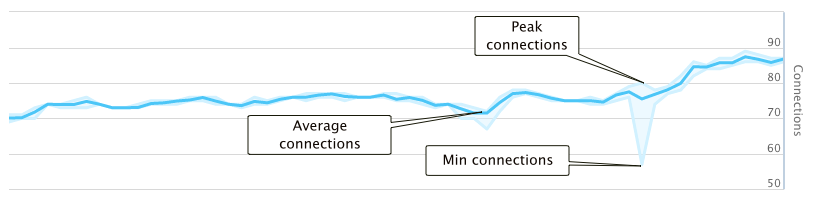
\includegraphics[width=0.8\textwidth]{figures/02_analysis/peak-conns}
    \caption{Peak connections metric. Source\cite{ably-peak}}
    \label{fig:peak-conns}
\end{figure}

However, all of the compared solutions are closed source and provide no means of self hosting. This leads to an intrinsic dependency on the companies that develop and maintain these platforms. This can be a problem for applications using these services if, for example, the pricing was suddenly changed, or the service was shut down entirely. A perfect example of this is when GoInstant was shut down and its customers were forced to switch to a different technology, one of these being PubNub, who offered a guide for migration\cite{pubnub-goinstant}.

\section{Requirement Analysis (Core System)}

After careful analysis of what is expected of the system, the following requirements are put in place. These requirements are split into two categories.

\subsection{Functional Requirements}
Functional requirements define the behaviour of the system.
\begin{itemize}
\item The system must be able to transmit messages between devices
\item The system must be able to deliver a single message to a single device
\item The system must be able to deliver a single message to several devices
\item The system must be able to receive messages from devices
\end{itemize}

\subsection{Non-functional Requirements}
Non-functional requirements define the properties of the system.
\begin{itemize}
\item The server side of the system must be easily horizontally scalable, ie. scaling by adding new instances
\item The server side of the system must be modular, so that the methods of receiving and sending messages can be easily replaced
\item The server side of the system must be testable
\item The server side of the system must be implemented so that it may run on the JVM\footnote{Java Virtual Machine} platform
\item The system must include a client library for these platforms: web, Android, iOS
\item Third party software, such as libraries, used by the system must be open source.
\end{itemize}

\section{Requirement Analysis (Sample Implementation)} \label{sec:sample-implementation-analysis}

In order to prove the system meets its requirements and works properly, a sample implementation of the highly modular parts of the system must be provided. This sample implementation must meet the following functional and non-functional requirements:

\subsection{Functional Requirements}\label{sec:s-impl-func-req}
Functional requirements define the behaviour of the system.
\begin{itemize}
\item The sample implementation must be able to deliver notifications and messages onto the Android platform.
\item The sample implementation must be able to deliver notifications and messages onto the iOS platform.
\item The sample implementation must be able to deliver notifications and messages onto the Web platform.
\item The sample implementation must be able to deliver notifications and messages onto the Java platform.
\end{itemize}

\subsection{Non-functional Requirements}
Non-functional requirements define the properties of the system.
\begin{itemize}
\item The sample implementation must include a module implementing database functionality for a relational database, eg. MySQL, PostgreSQL, MariaDB.
\end{itemize}

\section{Platform Analysis}

While the system will be designed in such a way that adding or removing supported platforms is simple, for the purposes of this thesis support of four of the most widely used platforms for both will be implemented.

\subsection{Android}
Android\footnote{Android <\url{https://www.android.com/}>} is a mobile operating system developed by Google\footnote{Google <\url{https://www.google.com/}>} widely used in smartphones, tablets, televisions, wearables and even automobiles. With around 80\% market share (see Figure ~\ref{fig:statista-mobile-market}) between mobile operating systems, it is indisputably one of the most important platforms on the market.

While development is lead mostly by Google, Android is an open source project. Its wide adoption by many manufacturers for different purposes is a direct result of this. The Android platform is based on a Linux kernel and apps are run using Android Runtime (ART)\footnote{ART <\url{https://source.android.com/devices/tech/dalvik/}>} created specifically for Android and uses the Dalvik Executable (Dex) bytecode specification. 

Development for Android can be done using the Android SDK, which allows the use of Java and Kotlin languages.

\begin{figure}[!ht]
	\centering
	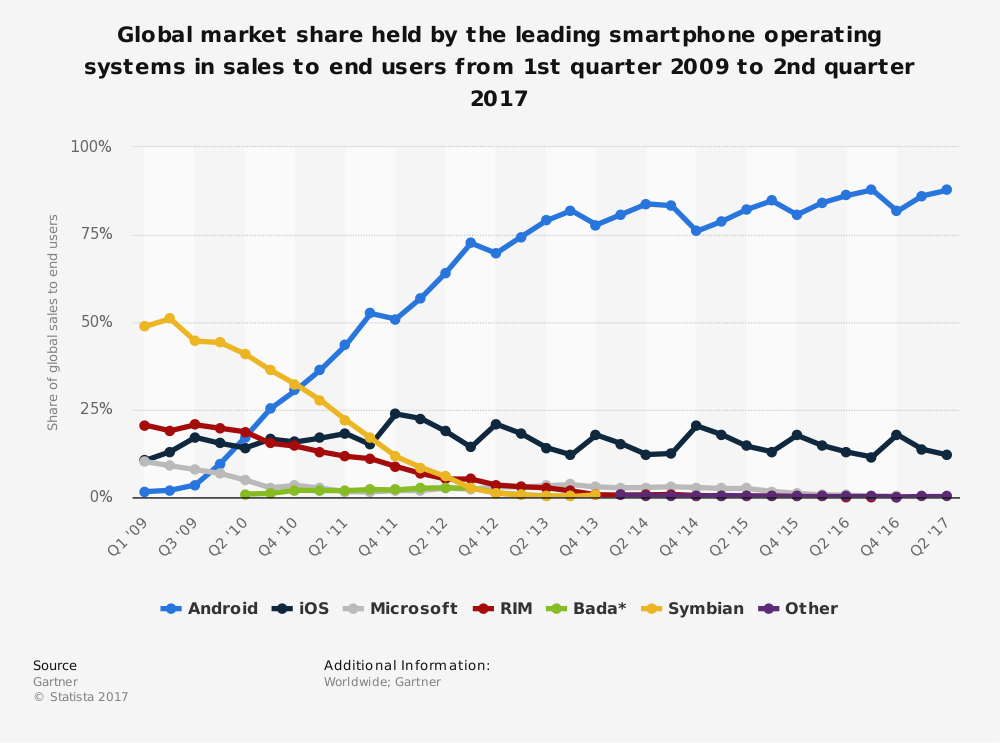
\includegraphics[width=0.8\textwidth]{figures/02_analysis/mobile-market}
    \caption{Global mobile OS market share in sales to end users. Source\cite{statista-mobile-share}}
    \label{fig:statista-mobile-market}
\end{figure}

\subsection{iOS}
iOS\footnote{iOS <\url{https://www.apple.com/lae/ios/ios-11/}>} is a mobile operating system developed by Apple\footnote{Apple <\url{https://www.apple.com/}>} used in smartphones, tablets, wearables and some other devices. Unlike Google's Android, iOS is a completely proprietary and closed source platform and can only be found on devices directly developed and sold by Apple. It is the second most popular mobile operating system (see Figure ~\ref{fig:statista-mobile-market}).

Development for iOS can be done using Xcode, Apple’s integrated development environment (IDE). While previously iOS apps were built mostly using Objective-C, Apple has been pushing forward their Swift\footnote{Swift <\url{https://developer.apple.com/swift/}>} language as the future of iOS (and MacOS) app development.

\subsection{Java}
Java\footnote{Java <\url{https://www.java.com/}>} is a popular language owned by Oracle\footnote{Oracle <\url{https://www.oracle.com/}>} that is compiled into Java bytecode, which can be run on any Java Virtual Machine (JVM), regardless of the underlying platform that the JVM is running on. It is one of the most popular platforms for developing enterprise server applications, owing to its large community support including extensive libraries, frameworks and platform independence.

\subsection{Web}
Frontend web applications based on HTML, CSS and JavaScript\footnote{HTML <\url{https://www.w3.org/wiki/The_web_standards_model_-_HTML_CSS_and_JavaScript/}>} as more full fledged and interactive applications, compared to the static web sites of the past, have been gaining on popularity. This is partly thanks to modern browsers and faster internet bandwidths and speeds and partly due to an explosion of powerful JavaScript-based frameworks and libraries. These applications have been moving some and in cases even most of application logic from backend servers to clients in web browsers. In order for these applications to be responsive and interactive, it is paramount to have realtime reliable communication with any components that are on a remote server.

\section{Analysis of Solutions for Implementation}
In order for the implementation of the core system to meet all of its requirements, a careful and well-informed choice of the proper tools is paramount. This section describes the chosen tools as well as elaborates on the reasons as to why these tools were chosen.
\subsection{Spring Boot}
Spring Boot\footnote{Spring Boot <\url{https://projects.spring.io/spring-boot/}>} is a JVM based framework for creating stand-alone production-grade applications based on the popular Spring Framework\footnote{Spring <\url{https://spring.io/}>}. Unlike most other enterprise Java frameworks, Spring Boot does not need a container to run in, as it includes an embedded one. This allows for easy and simple JAR (Java ARchive) based deployment.

Spring Boot is an opinionated framework, building on the idea of \textit{Convention over Configuration}. In essence, the idea behind this is to reduce the amount of configuration needed by having sensible defaults and using rules, or conventions, in naming and structure so that the framework may assume, based on these conventions, what it is supposed to do. A typical exam of this would be that a class called \textit{WelcomeController} would map to the \textit{'/welcome*'} URL\cite{convention-over-conf}.

Spring Boot, being based on the Spring Framework, has powerfull Inversion of Control (IoC) capabilites, also known as Dependency Injection (DI). IoC \texttt{"... is a process whereby objects define their dependencies, that is, the other objects they work with, only through constructor arguments, arguments to a factory method, or properties that are set on the object instance after it is constructed or returned from a factory method. The container then injects those dependencies when it creates the bean. This process is fundamentally the inverse, hence the name Inversion of Control (IoC), of the bean itself controlling the instantiation or location of its dependencies by using direct construction of classes, or a mechanism such as the Service Locator pattern."}\cite{ioc}

By delegating the creation and management of objects to the framework, IoC reduces the dependency of components on one another while still allowing them to interact and allows for more modularity, as it is the framework at runtime who decides which instances will be injected, typically by building what is called a Dependency Graph.

Spring Boot projects can be managed by either of the two most popular JVM build automation and dependency management tools: Maven and Gradle.
\subsubsection*{Maven}
Maven\footnote{Apache Maven <\url{https://maven.apache.org/}>} is one of the most popular JVM build automation and dependency management tools. Maven's configuration is based on XML files. It manages the project's dependencies (third-party modules and libraries) and defines the build and execution order of different tasks. Maven also downloads the project's dependencies from online repositories, which are defined in the configuration, and caches them on the local machine.

Maven is distributed as open source under the Apache License, Version 2.0\footnote{Apache License 2.0 <\url{https://www.apache.org/licenses/}>}.

\subsubsection*{Gradle}
Gradle\footnote{Gradle <\url{https://gradle.org/}>} has, over the past few years, become a strong competitor to Maven and gained great popularity\cite{maven-gradle}. Like Maven, Gradle is a build automation and dependency management tool. However, it uses a Groovy-based DSL (Domain-Specific Language) for its configuration. This leads to shorter and more readable configuration files, while at the same time providing more flexibility and even scripting options. Like Maven, Gradle also downloads dependencies from online repositories and stores them on the local machine.

When it comes to performance, thanks to its advanced and modern techniques, Gradle builds are much faster compared to Maven (see Figure ~\ref{fig:maven-gradle-speed}).

\begin{figure}[!ht]
	\centering
	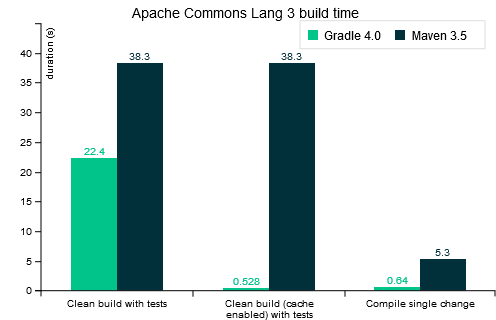
\includegraphics[width=0.8\textwidth]{figures/02_analysis/maven-gradle-speed}
    \caption{Maven and Gradle build time comparison. Source\cite{maven-vs-gradle}}
    \label{fig:maven-gradle-speed}
\end{figure}

Thanks to the Gradle's learning curve, ease of use and advanced features, Gradle is the default build tool for Google's Android OS.

Both Gradle and Spring Boot are distributed as Open Source software under the same license as Maven, the Apache License (ASL), Version 2.0 \footnote{Apache License 2.0 <\url{https://www.apache.org/licenses/}>}.

\subsubsection*{Build Tool Conclusion}
After careful evaluation of the available build and dependency management tools, including their features, drawbacks and things such as active community support, extensibility and thorough documentation, among others, the selected tool for the implementation part of this thesis shall be Gradle.

\subsubsection*{Why not use a server-less solution?}
Server-less solutions are inherently dependent on the platform they are ran on. This has the same large disadvantages as non-self-hosted services discussed in Section \ref{sec:similar-solutions} \nameref{sec:similar-solutions}, mainly dependence on whoever runs the platform and the possibility of great impacts to the application in case of price changes or service termination.

\subsection{Testing Framework}
In order to create tests for the system's code, a powerful testing framework is needed.
\subsubsection{JUnit}
JUnit\footnote{JUnit <\url{http://junit.org/junit5/}>} is one of the most popular JVM-based testing framework. Since the JUnit 5 version, it has been split into three main modules, The JUnit Platform, JUnit Jupiter and JUnit Vintage.

The JUnit Platform \texttt{"serves as a foundation for launching testing frameworks on the JVM. It also defines the TestEngine API for developing a testing framework that runs on the platform. Furthermore, the platform provides a Console Launcher to launch the platform from the command line and build plugins for Gradle and Maven as well as a JUnit 4 based Runner for running any TestEngine on the platform."}\cite{junit}

On top of providing the basis for running other testing frameworks, JUnit also provides its own solution for writing tests, which resides in the JUnit Jupiter module.

JUnit is Open Source software released under the Eclipse Public License (EPL) 1.0\footnote{EPL 1.0 <\url{https://opensource.org/licenses/EPL-1.0}>}.

\subsubsection{Spock Framework}
Spock\footnote{Spock Framework <\url{http://spockframework.org/}>} is a powerful all-round testing framework for the JVM platform. Based on the Groovy\footnote{Apache Groovy <\url{http://groovy-lang.org/}>} language and JUnit, it aims to put together the plethora of test libraries available into a comprehensive and easy to use framework. 

Thanks to its use of Groovy DSL, Spock boasts an easy to understand and expressive specification language. On top of basic testing, some of its more advanced features include powerful Mocking APIs, class Stubbing, Data Driven Testing and Interaction Driven Testing and its Spring Module provides seamless integration with the Spring TestContext Framework\cite{spock}.

Spock Framework is Open Source software distributed under the Apache License (APL) 2.0\footnote{APL 2.0 <\url{https://www.apache.org/licenses/LICENSE-2.0}>}

\subsection{Database technology}
Since the system needs to persistently store, alter and access data, a database system is a proper solution. One of the most commonly used methods of accessing database storage in Java applications is the usage of an ORM (Object-Relational Mapping) framework, arguably the most popular one being Hibernate\footnote{Hibernate <\url{http://hibernate.org/}>}.

Hibernate provides abstraction from the concrete database implementation, along with its own query language, HQL (Hibernate Query Language), which allows for more flexibility and interchangeability when it comes to the database software in use. Hibernate's ORM implementation is also an implementation of the Java Persistence API (JPA)\cite{hibernate-orm}.

On top of powerful ORM for SQL databases, Hibernate also provides Hibernate OGM, a powerful JPA implementation for NoSQL database systems, including first party implementations for Infinispan, MongoDB and Neo4j and community-maintained dialects for Cassandra, CouchDB, EhCache, Apache Ignite and Redis\cite{hibernate-ogm}.

Hibernate is Free Software distributed under the GNU Lesser General Public License (LGPL) 2.1\footnote{LGPL 2.1 <\url{https://www.gnu.org/licenses/old-licenses/lgpl-2.1.html/}>} or Apache License (ASL), Version 2.0\footnote{ASL 2.0 <\url{https://www.apache.org/licenses/LICENSE-2.0.html/}>} licenses.

The aim of the system implemented as part of this thesis is to provide as much freedom, flexibility and modularity to the its users\footnote{Users here meaning those who would self-host the system, not the end users of any application using the system}. For this reason, the system should be designed in such a way that it is easy to switch out the end database layer, including support for both SQL and NoSQL databases, and create custom implementations.

\section{Analysis of Solutions for Sample Implementation}
In order to prove the system meets its requirements and works properly, a sample implementation of the highly modular parts of the system must be provided. The requirements for the sample implementation are listed in Section \ref{sec:sample-implementation-analysis} \nameref{sec:sample-implementation-analysis}.

\subsection{Firebase Cloud Messaging}
Firebase Cloud Messaging (FCM)\footnote{FCM <\url{https://firebase.google.com/docs/cloud-messaging/}>} is a multi-platform messaging solution by Google\footnote{Google <\url{https://google.com}>}. FCM is the successor to the Google Cloud Messaging (GCM)\footnote{GCM <\url{https://developers.google.com/cloud-messaging/}>} platform, that was aimed mainly at the Android, iOS and Google Chrome platforms. On top the platform support of GCM, FCM adds support for the Web, C++ and Unity platform.

On top of a first party server library for NodeJS, FCM provides powerful HTTP and XMPP (Extensible Messaging and Presence Protocol) APIs.

\subsubsection*{Key Features\cite{fcm}}
\begin{itemize}
\item Support for Android, iOS, Web, C++ and Unity platforms.
\item Unlimited number of messages, with up to 4kB of data each.
\item Support for Notification messages, which display a notification at the target device to the user.
\item Support for Data messages, which are only handled in the background of the app on the target device.
\item Normal and High priority message setting.
\item Message Time to Live (TTL).
\item HTTP and XMPP APIs.
\item Free.
\end{itemize}

Firebase Cloud Messaging shall be used in the sample implementation to relay messages onto the Android, iOS and Web platforms. 

In order to simplify the use of FCM from the system a proper client library should be used. While there are no first party Java libraries, there are several community-maintained ones, two of which are compared below.

\subsubsection{FcmJava}
FcmJava\footnote{FcmJava <\url{https://github.com/bytefish/FcmJava}>} is a community-maintained Java library for communication with the FCM API. It provides object-oriented encapsulation of the FCM APIs. At the time of selecting the tools for the sample implementation (14. 1. 2018), FcmJava does not support the new FCM HTTP v1 API, but uses the Legacy HTTP Cloud Messaging, however support for the FCM HTTP v1 API is planned in the 3.0 milestone\cite{fcmJava}.

\subsubsection{Pushraven}
Pushraven\footnote{Pushraven <\url{https://github.com/Raudius/Pushraven}>} is a community-maintained Java library for communicating with the FCM API. It provides a nicely designed object-oriented encapsulation of the FCM APIs, that is simple to use and very easy to read. On 1. 12. 2017, the main auther of Pushraven, Raudius, released a fully updated version of the library with support of the new FCM HTTP v1 API\cite{pushraven-new-api}.

\subsubsection*{FCM library conclusion}
Due to its good design, ease of use, fast update intervals and support of the more modern FCM HTTP v1 APIs, the library used in the sample implementation will be Pushraven.